\lecdate{24.04.2017}
\section{Arithmetik in Prolog}
Arithmetische Ausdrücke werden mit dem Operator \lstinline$is$ ausgewertet. Dabei muss die rechte Seite instantiiert sein.
\cparagraph{Beispiel}$ $
\begin{lstlisting}[language=Prolog]
?- X is 3+4.
X=7.
?- 10 is 3+4.
false.
?- 2 is 1+X
Fehler!!!
f(X,Y):- Y=3*X+1	% Falsch! = ist Unifikationsoperator, keine Funktionszuweisung
f(1,Y).
Y=3*1+1.
\end{lstlisting}

\subsection{Vergleichsoperatoren}
\begin{tabular}{c l l}
Operator & Bedeutung & Beispiel\\\hline
\lstinline$==$ & identisch & \lstinline$p(X) == p(X)$\\
\lstinline$\==$ & nicht identisch & \lstinline$p(X) \== p(Y)$\\
\lstinline$=$ & unifizierbar & \lstinline$p(X) = p(Y)$\\
\lstinline$\=$ & nicht unifizierbar & \lstinline$p(X) \= q(X)$\\
\lstinline$=:=$ & arithmetisch gleich & \lstinline$2 =:= 1+1$\\
\lstinline$=\=$ & arithmetisch ungleich & \lstinline$3 =\= 1+1$
\end{tabular}\\
In Prädikaten können Operatorsymbole wie $+, -, *, /, \hat{\,}$ verwendet werden, um arithmetische Ausdrücke zu zerlegen. Prolog berücksichtigt dabei die Priorität der Operatoren.
\cparagraph{Beispiel}$ $
\begin{lstlisting}[language=Prolog]
?- x + 3*y + x*2 = A + B + C.
A=x, B=3*y, C=x*2.
?- 2*x + 3*y = A + B * C.
A=2*x, B=3, C=y
?- 2*x + y + z = A + B % nicht eindeutig!
\end{lstlisting}

\subsection{Anwendungen}
\subsubsection{Symbolisches Differenzieren}
Ziel: Wir wollen ein Prädikat \lstinline$diff/3$ (3-Stelliger Operator) definieren, mit dem Polynome symbolisch differenziert werden können.
\cparagraph{Beispiel} $ $
\begin{lstlisting}[language=Prolog]
diff(3*x^2+5x-2 , x , D).
D = 6*x+5.
\end{lstlisting}
\begin{lstlisting}[language=Prolog]
d(X,X,1).
d(C,X,0) :- atomic(C), C\==X.

?- d(x,x,D).
D = 1.
?- d(c,x,D).
D = 0.
?- d(x+y, x+y, D).
D = 1.

% weitere Ableitungsregel (Ableitung negativer Funktion):
d(-F,X,-DF) :- d(F,X,DF).

?- d(-x,x,D).
D = -1.

% weitere Ableitungsregel (Ableitung mit führender Konstante):
d(C*F,X,C*DF) :- d(C,X,0), d(F,X,DF).

?- d(3*x,x,D).
D = 3*1.

% weitere Ableitungsregel (Kettenregel):
d(F+G,X,DF+DG) :- d(F,X,DF), d(G,X,DG).
d(F-G,X,DF-DG) :- d(F,X,DF), d(G,X,DG).

?- d(3*x+5,x,D).
D = 3*1+0.

% weiter Ableitungsregel (einfache Ableitung): 
d(F^N,X,N*F^M):- number(N), M is N-1, d(F,X,DF).
\end{lstlisting}

\subsubsection{Vereinfachen von arithmetischen Ausdrücken}
Idee: Wir definieren elementare Vereinfachungsregeln und vereinfachen rekursiv.\\
Elementare Vereinfachungsregeln:
\begin{lstlisting}[language=Prolog]
s0(1*X,X).
s0(X*1,X).
s0(0+X,X).
s0(X+0,X).
%...
s0(X,X).	% Lösung zu folgendem Problem
\end{lstlisting}
Problem: Wenn ein Term bereits vereinfacht ist, liefert \lstinline$s0 false$. Zum Beispiel \lstinline$s0(x,X)$.\\
Lösung: Regel \lstinline$s0(X,X).$ am Ende hinzufügen (wenn keine der Regeln greift, ist Term schon vereinfacht).\\
Um Ausdrücke zu vereinfachen, die aus mehreren Termen bestehen, wenden wir die Vereinfachung rekursiv auf jeden Term an und vereinfachen das Ergebnis. Zum Beispiel: Ausdruck $1*x+3*1+0$
\begin{center}
\begin{tikzpicture}
\node at (-3.5,2) {$\underset{A}{\underline{1*x+3*1}}+\underset{B}{\underline{0}}$};
\draw (-2.5,1.5) -- (-2,0.5) node[below]{$0$};
\draw (-4,1.5) -- (-5,0.5) node[below]{$\underset{A}{\underline{1*x}}+\underset{B}{\underline{3*1}}$};
\draw (-5.5,-0.5) -- (-6,-1.5) node[below]{$x$};
\draw (-4.5,-0.5) -- (-4,-1.5) node[below]{$3$};
\node [left] at (-7,0) {Ergebnis: $x+3$};
\node [align=right, left] at (-7,2) {Ergebnis: $x+3+0$\\Vereinfachen gibt: $x+3$};
\end{tikzpicture}
\end{center}

\section{Listen}
\lecdate{08.05.2017}
Listen sind induktiv definiert:
\begin{itemize}
\item \lstinline$[]$ ist die leere Liste
\item Wenn \lstinline$H$ ein Element und $T$ eine Liste sind, dann ist \lstinline$[H|T]$ eine Liste die aus dem Kopf \lstinline$H$ und der restlichen Liste \lstinline$T$ besteht.
\end{itemize}
Alternativ kann eine Liste in der Form \lstinline$[x1, ..., xn]$ aufgeschrieben werden.
\cparagraph{Beispiel} Listen sind:
\begin{itemize}
\item \lstinline$[a,b,c]$
\item \lstinline$[a|[b,c]]$
\item \lstinline$[a,b,c,1,2,[u,v]]$
\end{itemize}
\subsection{Suche (member)}
Als Beispiel für ein Prädikat auf einer Liste definieren wir das member-Prädikat:
\begin{lstlisting}[language=Prolog]
member(X, [X|_]).	% Element ist im Kopf, _ kann auch die leere Liste sein.
member(X, [_|T]):- member (X,T).	% Element in der Tail-Liste suchen.
\end{lstlisting}
\cparagraph{Beispiel} Suchbaum für die Anfrage \lstinline$member(b,[a,b,c])$:
\begin{center}
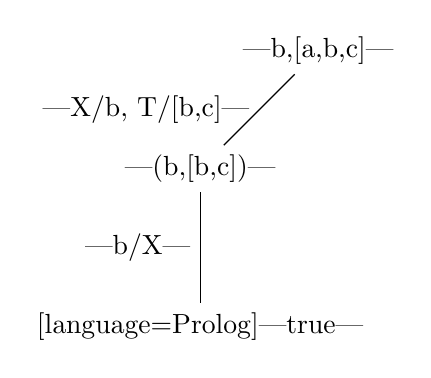
\begin{tikzpicture}[align=center]
\node (v1) at (0,0) {\lstinline|b,[a,b,c]|};
\node (v2) at (-1.5,-1.5) {\lstinline|(b,[b,c])|};
\draw (v1) -- node[pos=.5, left]{\lstinline|X/b, T/[b,c]|} (v2);
\node (v3) at (-1.5,-3.5) {\lstinline[language=Prolog]|true|};
\draw (v2) -- node[pos=.5, left]{\lstinline|b/X|} (v3);
\end{tikzpicture}
\end{center}

\subsection{Konkatenieren (append)}
Weiteres Listenelement: \lstinline$append/3$\\
\lstinline$append(L1, L2, L3)$ ist wahr genau dann, wenn die Verkettung der Listen L1, L2 und L3 gleich ist.
\cparagraph{Beispiel}
\begin{itemize}
\item \lstinline$append([a,b,c], [d,e,f], L)$ liefert \lstinline$L=[a,b,c,d,e,f]$.
\item \lstinline$append([a,b,c], L, [a,b,c,d,e,f])$ liefert \lstinline$L=[d,e,f]$.
\item \lstinline$append(L1, L2, [a,b])$ liefert:\\
\lstinline$L1=[], L2=[a,b];$\\
\lstinline$L1=[a], L2=[b];$\\
\lstinline$L1=[a,b], L2=[].$
\end{itemize}














